\documentclass[a4paper,12pt]{article}
\usepackage[utf8]{inputenc}
\usepackage[english]{babel}
\usepackage{graphicx}
\usepackage{geometry}
\usepackage{listings}
\usepackage{xcolor}
\usepackage{hyperref}
\usepackage{tikz}
\usetikzlibrary{shapes, arrows, positioning}

% Cấu hình hiển thị code
\definecolor{codegreen}{rgb}{0,0.6,0}
\definecolor{codegray}{rgb}{0.5,0.5,0.5}
\definecolor{codepurple}{rgb}{0.58,0,0.82}
\definecolor{backcolour}{rgb}{0.95,0.95,0.92}

\lstdefinestyle{mystyle}{
    backgroundcolor=\color{backcolour},   
    commentstyle=\color{codegreen},
    keywordstyle=\color{magenta},
    numberstyle=\tiny\color{codegray},
    stringstyle=\color{codepurple},
    basicstyle=\ttfamily\footnotesize,
    breakatwhitespace=false,         
    breaklines=true,                 
    captionpos=b,                    
    keepspaces=true,                 
    numbers=left,                    
    numbersep=5pt,                  
    showspaces=false,                
    showstringspaces=false,
    showtabs=false,                  
    tabsize=2
}

\lstset{style=mystyle}

\geometry{
  top=2cm,
  bottom=2cm,
  left=2.5cm,
  right=2.5cm
}

\title{\textbf{Practical Work 2: RPC File Transfer}}
\author{Le Quy Ton \\ 23BI14425}
\date{\today}

\begin{document}

\maketitle

\section{Introduction}
The objective of this practical work is to upgrade a TCP file transfer system to use Remote Procedure Calls (RPC). We utilize Python's \texttt{xmlrpc} library to implement a file transfer service where binary data is encoded in Base64 and transmitted in chunks.

\section{Design of the RPC Service}
To handle file transfers effectively over XML-RPC (which is text-based), we designed the service with three specific remote procedures. This ensures that large files do not consume excessive memory and allows for basic session management.

The service exposes the following methods:

\begin{itemize}
    \item \textbf{\texttt{start\_transfer(filename, filesize)}:} 
    Initializes the transfer on the server. The server checks if the file size is valid, resolves naming conflicts, and opens a file handle for writing.
    
    \item \textbf{\texttt{send\_chunk(chunk\_b64)}:} 
    Receives a Base64-encoded string representing a part of the file. The server decodes it back to binary and writes it to the active file handle.
    
    \item \textbf{\texttt{finish()}:} 
    Finalizes the transfer. The server closes the file handle and verifies if the received size matches the expected size.
\end{itemize}

\subsection{Transfer Sequence Diagram}
Below is the sequence of operations between the Client and the Server:

\begin{center}
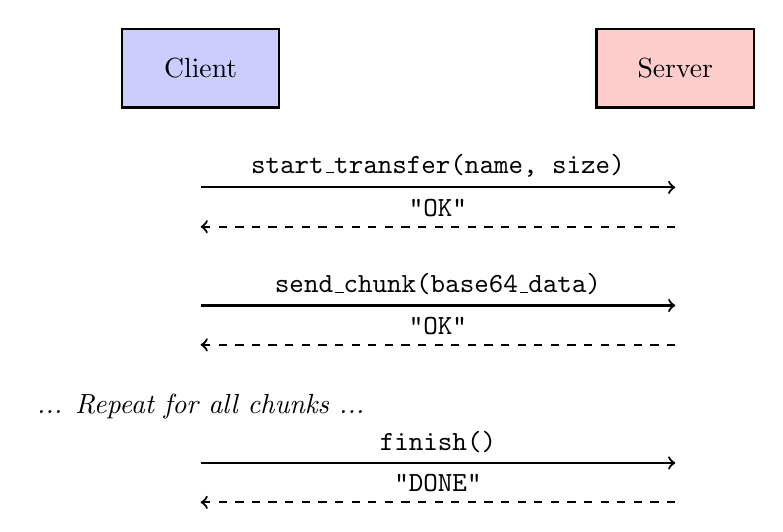
\begin{tikzpicture}[node distance=4cm, auto, thick]
    % Nodes
    \node (client) [rectangle, draw, fill=blue!20, minimum height=1cm, minimum width=2cm] {Client};
    \node (server) [rectangle, draw, fill=red!20, minimum height=1cm, minimum width=2cm, right=of client] {Server};
    
    % Timeline
    \draw[->] ([yshift=-1cm]client.south) -- ([yshift=-1cm]server.south) node[midway, above] {\texttt{start\_transfer(name, size)}};
    \draw[dashed, ->] ([yshift=-1.5cm]server.south) -- ([yshift=-1.5cm]client.south) node[midway, above] {\texttt{"OK"}};
    
    \draw[->] ([yshift=-2.5cm]client.south) -- ([yshift=-2.5cm]server.south) node[midway, above] {\texttt{send\_chunk(base64\_data)}};
    \draw[dashed, ->] ([yshift=-3.0cm]server.south) -- ([yshift=-3.0cm]client.south) node[midway, above] {\texttt{"OK"}};
    
    \node at ([yshift=-3.5cm]client.south) [below] {\textit{... Repeat for all chunks ...}};
    
    \draw[->] ([yshift=-4.5cm]client.south) -- ([yshift=-4.5cm]server.south) node[midway, above] {\texttt{finish()}};
    \draw[dashed, ->] ([yshift=-5.0cm]server.south) -- ([yshift=-5.0cm]client.south) node[midway, above] {\texttt{"DONE"}};

\end{tikzpicture}
\end{center}

\section{System Organization}
The system is organized into a Client-Server architecture using the HTTP protocol as the transport layer for XML-RPC.

\begin{itemize}
    \item \textbf{Client Side:} Reads the source file, encodes binary data to Base64 to ensure safe transmission over XML, and sends it sequentially.
    \item \textbf{Server Side:} Listens on port 8000. It manages a state machine (using a dictionary \texttt{\_state}) to keep track of the current file being written, ensuring thread safety with locks.
    \item \textbf{Storage:} Files received by the server are stored in a dedicated directory named \texttt{received\_files/}.
\end{itemize}

\begin{figure}[h]
    \centering
    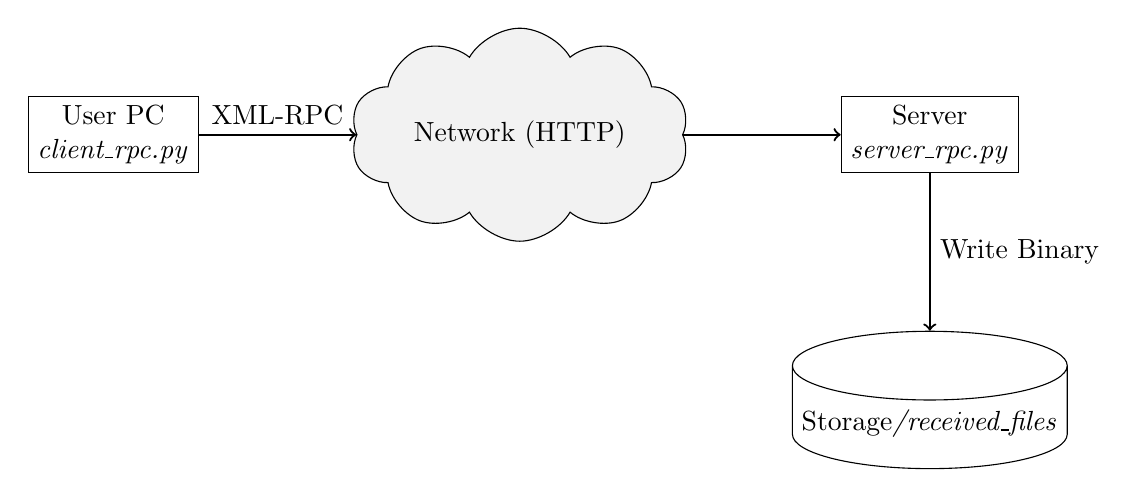
\begin{tikzpicture}[node distance=2cm]
    \node (pc) [draw, rectangle, align=center] {User PC \\ \textit{client\_rpc.py}};
    \node (internet) [cloud, draw,cloud puffs=10,cloud puff arc=120, aspect=2, right=of pc, fill=gray!10] {Network (HTTP)};
    \node (serv) [draw, rectangle, align=center, right=of internet] {Server \\ \textit{server\_rpc.py}};
    \node (disk) [cylinder, shape border rotate=90, draw, aspect=0.25, below=of serv] {Storage \\ \textit{/received\_files}};

    \draw[->, thick] (pc) -- (internet) node[midway, above] {XML-RPC};
    \draw[->, thick] (internet) -- (serv);
    \draw[->, thick] (serv) -- (disk) node[midway, right] {Write Binary};
    \end{tikzpicture}
    \caption{System Architecture}
\end{figure}

\section{Implementation}

\subsection{Server Side Implementation}
The server uses \texttt{SimpleXMLRPCServer}. Key logic for handling chunks is shown below:

\begin{lstlisting}[language=Python, caption=Server Logic for Receiving Chunks]
def send_chunk(chunk_b64):
    with _state_lock:
        if not _state["active"]:
            return "ERROR: no active transfer"
        try:
            # Decode Base64 back to binary
            data = base64.b64decode(chunk_b64)
            _state["file_obj"].write(data)
            _state["received"] += len(data)
        except Exception as e:
            return f"ERROR: write failed: {e}"
        return "OK"
\end{lstlisting}

\subsection{Client Side Implementation}
The client reads the file in 64KB chunks, encodes them, and sends them via the proxy.

\begin{lstlisting}[language=Python, caption=Client Loop for Sending File]
# Connect to server
proxy = xmlrpc.client.ServerProxy("http://localhost:8000/", allow_none=True)
proxy.start_transfer(basename, filesize)

CHUNK = 64 * 1024
with open(filename, "rb") as f:
    while True:
        chunk = f.read(CHUNK)
        if not chunk:
            break
        # Encode binary chunk to Base64 string
        b64 = base64.b64encode(chunk).decode()
        proxy.send_chunk(b64)

result = proxy.finish()
print("Transfer complete:", result)
\end{lstlisting}

\section{Conclusion}
In this practical work, I successfully transformed a raw TCP file transfer system into a Remote Procedure Call (RPC) based application. By utilizing Python's \texttt{xmlrpc} library, the complexity of socket management was abstracted, allowing the client to interact with the server through defined method calls.

Key achievements include:
\begin{itemize}
    \item \textbf{Protocol Abstraction:} Moved from stream-based communication to a function-call model.
    \item \textbf{Binary Handling:} Successfully implemented Base64 encoding/decoding to transport binary files (images, executables) over the text-based XML protocol.
    \item \textbf{Chunked Transfer:} Implemented a chunk-based mechanism to handle large files without exhausting system memory.
\end{itemize}

While RPC introduces some overhead due to XML parsing and Base64 encoding compared to raw TCP, it significantly simplifies the development process and code readability.

\end{document}
